\documentclass[a4paper]{article}

\usepackage{fullpage} % Package to use full page
\usepackage{parskip} % Package to tweak paragraph skipping
\usepackage{tikz} % Package for drawing
\usepackage{amsmath}
\usepackage{hyperref}
\usepackage{verbatimbox}
\usepackage{listings}
\usepackage{xcolor}
\usepackage{subfigure}

\definecolor{mygreen}{rgb}{0,0.6,0}
\definecolor{mygray}{rgb}{0.5,0.5,0.5}
\definecolor{mymauve}{rgb}{0.58,0,0.82}
\lstset{ %
  backgroundcolor=\color{white},   % choose the background color
  basicstyle=\footnotesize,        % size of fonts used for the code
  numberstyle=\tiny,
  breaklines=true,                 % automatic line breaking only at whitespace
  captionpos=b,                    % sets the caption-position to bottom
  commentstyle=\color{mygreen},    % comment style
  escapeinside={\%*}{*)},          % if you want to add LaTeX within your code
  keywordstyle=\color{blue},       % keyword style
  stringstyle=\color{mymauve},     % string literal style
}

\title{CSCE 569: Homework 1}
\author{Nick Tyler}
\date{02/09/18}

\begin{document}

\maketitle

\section*{Matrix Matrix Multiplication}
Mathematically matrix multiplication between two matrices, A and B size M$\times$L and L$\times$N, to form the resultant matrix with size M$\times$N and the elements defined by: $c_{ij} = \sum_{k} a_{ik}b_{kj}$ 
The row major multiplication is made into an algorithm as seen below, where the new element of C is calculated by taking the values of the i'th row of matrix A and j'th column of matrix B multiplying them together and then adding them to a temporary value. The row of A and column of B are then walked through, multiplied together, and then summed to get the total value.

\begin{lstlisting}[language=C++]
for (i = 0; i < N; i++){ // Loop over cols
  for (j = 0; j < M; j++) { // Loop over rows
    float temp = 0.0; // Create temp to for new element
    for (w = 0; w < K; w++) // Walk through the row/column
      temp += A[i * K + w] * B[w * M + j]; // Add the product of elements
    C[i * M + j] = temp; // Put element into output matrix
  }
}
\end{lstlisting}
Depending on how the matrix is stored in memory the algorithm must be modified slightly. The skeleton of the algorithm stays the same, the only change is to how the elements of A and B are accessed in memory. This modification to the fifth line of the code can be seen below.

\begin{lstlisting}[language=C++]
temp += A[i * K + w] * B[w * M + j]; // A Row, B Row
temp += A[w * K + i] * B[w * M + j]; // A Col, B Row
temp += A[w * K + i] * B[j * M + w]; // A Row, B Col
temp += A[i * K + w] * B[j * M + w]; // A Col, B Col
\end{lstlisting}

\section*{Matrix Vector Multiplication}
Matrix vector multiplication is just a special case of matrix multiplication where a matrix A of size M$\times$N is multiplied with a matrix B of size N$\times$1, resulting in a matrix C of size M$\times$1. Again the elements of C are defined similarly with a summation over the products of the two as shown: $c_{i} = \sum_{k} a_{ik}b_{k}$
And with an algorithm, as:
\begin{lstlisting}[language=C++]
for (i = 0; i < M; i++) { // Loop over rows
  float temp = 0.0; // Create temp to for new element
  for (j = 0; j < N; j++) { // Loop over cols
    temp += A[i * N + j] * B[j];  // Add the product of elements
  }
  C[i] = temp; // Put element into output vector
}
\end{lstlisting}

Changing how to access the elements of A is all that is needed to go from row to column storage.

\begin{lstlisting}[language=C++]
temp += A[i * N + j] * B[j];  // A Row major
temp += A[j * N + i] * B[j];  // A Col Major
\end{lstlisting}


\section*{Histogram}

A histogram of an image takes the color values of each pixel and tallies up how many of each value are in the image. The basic algorithm is to find the color value present, and add one to the count for that bin. 
\begin{lstlisting}[language=C++]
  for (int i = 0; i < src.cols; i++) { // Loop over cols
    for (int j = 0; j < src.rows; j++) { // Loop over rows
      k = src.at<uchar>(j, i); // Get current value
      histogram[k] += 1; // Add one to the histogram 
    }
  }
\end{lstlisting}

\section*{Smoothing}

To smooth an image information from a pixel the surrounding pixels is taken in, and the surrounding pixels are given a weight from a matrix known as a filter. The weighted average of the pixel and surrounding pixels is then calculated and the new pixel value is places in the output image.

\begin{lstlisting}[language=C++]
for (int j = 1; j < src.rows - 1; j++) { // Loop over rows
  for (int i = 1; i < src.cols - 1; i++) { // Loop over cols
    unsigned int value[3]; // Setup temporary value for new pixels
    for (int x = 0; x < 3; x++) { // Loop over pixels blue, green, red
      for (int a = -1; a < 2; a++) { // Per-mutate over the filter matrix
        for (int b = -1; b < 2; b++) {
          // Store temporary value as current/surrounding pixels times filter
          value[x] +=
            src.at<cv::Vec3b>(j + b, i + a)[x] * filter[a + 1][b + 1];
        }
      }
      value[x] /= weight; // Take the average knowing the weight of filter
      // If the value is negative place a 0, if it is too large place largest pixel value (265)
      value[x] = ((value[x] < 0) ? 0 : value[x]); 
      value[x] = ((value[x] > MAX_COLOR) ? MAX_COLOR : value[x]); 
      dst.at<cv::Vec3b>(j, i)[x] = value[x]; //Place into proper value of new image
    }
  }
}
\end{lstlisting}

\section*{Performance}
All performance results are from my personal computer running Ubuntu 17.10, Artful, with 16GB of ram and an intel core i7-3770, running at 3.4GHz and a peak performance per core of 13.6Gflop/s.

\begin{verbnobox}[\footnotesize]
Architecture:        x86_64
CPU op-mode(s):      32-bit, 64-bit
Byte Order:          Little Endian
CPU(s):              8
On-line CPU(s) list: 0-7
Thread(s) per core:  2
Core(s) per socket:  4
Socket(s):           1
NUMA node(s):        1
Vendor ID:           GenuineIntel
CPU family:          6
Model:               58
Model name:          Intel(R) Core(TM) i7-3770 CPU @ 3.40GHz
Stepping:            9
CPU MHz:             3400.264
CPU max MHz:         3900.0000
CPU min MHz:         1600.0000
BogoMIPS:            6800.52
Virtualization:      VT-x
L1d cache:           32K
L1i cache:           32K
L2 cache:            256K
L3 cache:            8192K
NUMA node0 CPU(s):   0-7
\end{verbnobox}

The programs for Matrix Matrix and Matrix Vector multiplication were tested both with and without gcc optimization's. With gcc optimization's enabled (-O3) the compiler will attempt to optimize the executable for speed. There are many flags which are enabled with optimization but most likely one of the optimization's involving loop unraveling or vectorization are what helps to speed up the results. All the information on what the optimizations are and all the flags enabled was found at the \href{https://gcc.gnu.org/onlinedocs/gcc/Optimize-Options.html}{online gcc optimization manual}.

The performance for matrix multiplication can be seen in the graphs below. The worst performance came from A column major and B row major at a size of 2048 with no optimization. Even with optimization's enabled it was not fast in it's execution time. However storing the matrices as column major gives the best performance, it is the fastest method both with and without optimization's enabled. The column major representation was also the most efficient at over 86\% efficiency for both the matrix of 1024 and 2048. All times and the efficiency can be seen in the tables below.

With matrix vector multiplication the row major matrix is faster than both implementations of the optimized column major matrix. This probably comes from the fact that by doing row major element searches in both the matrix and vector are continuous instead of having to access elements out of order.

For the histogram the execution time was 4.999876ms giving a value of 157.290300 MegaFlops and a efficiency of 0.01157. For the Smoothing the time was 64.999819ms giving a value of 108.890888 MegaFlops and an efficiency of 0.008007.

\begin{tabular}{|c|c|c|c|c|c|c|}
\hline
 & Time 1024 (ms) & Gflops 1024 & efficiency 1024 \\ \hline
mm (row, row) -O0 & 6456.00009 & 1.663168849 & 0.122291827 \\ \hline
mm (row, col) -O0 & 6157.999992 & 1.7436535 & 0.128209816 \\ \hline
mm (col, row) -O0 & 12727.99993 & 0.843606089 & 0.062029859 \\ \hline
mm (col, col) -O0 & 2621.999979 & 4.09512522 & 0.301112149 \\ \hline
mm (row, row) -O3 & 6347.000122 & 1.691731217 & 0.124392001 \\ \hline
mm (row, col) -O3 & 6341.00008 & 1.693331983 & 0.124509705 \\ \hline
mm (col, row) -O3 & 13778.99981 & 0.779259626 & 0.057298502 \\ \hline
mm (col, col) -O3 & 828.000069 & 12.96789534 & 0.953521717 \\ \hline
\end{tabular}

\begin{tabular}{|c|c|c|c|c|c|c|}
\hline
 & Time 2048 (ms) & Gflops 2048 & efficiency 2048 \\ \hline
mm (row, row) -O0 & 140391 & 0.611857925 & 0.044989553 \\ \hline
mm (row, col) -O0 & 117842 & 0.728936592 & 0.053598279 \\ \hline
mm (col, row) -O0 & 166770.9999 & 0.51507364 & 0.037873062 \\ \hline
mm (col, col) -O0 & 21154.00004 & 4.060666812 & 0.298578442 \\ \hline
mm (row, row) -O3 & 63353.99985 & 1.355863026 & 0.099695811 \\ \hline
mm (row, col) -O3 & 58741.00018 & 1.46234054 & 0.10752504 \\ \hline
mm (col, row) -O3 & 129912.9999 & 0.6612067 & 0.04861814 \\ \hline
mm (col, col) -O3 & 7271.000147 & 11.81396564 & 0.868673944 \\ \hline
\end{tabular}

\pagebreak
\begin{figure}
\vfill
\subfigure[Matrix Matrix Performance]{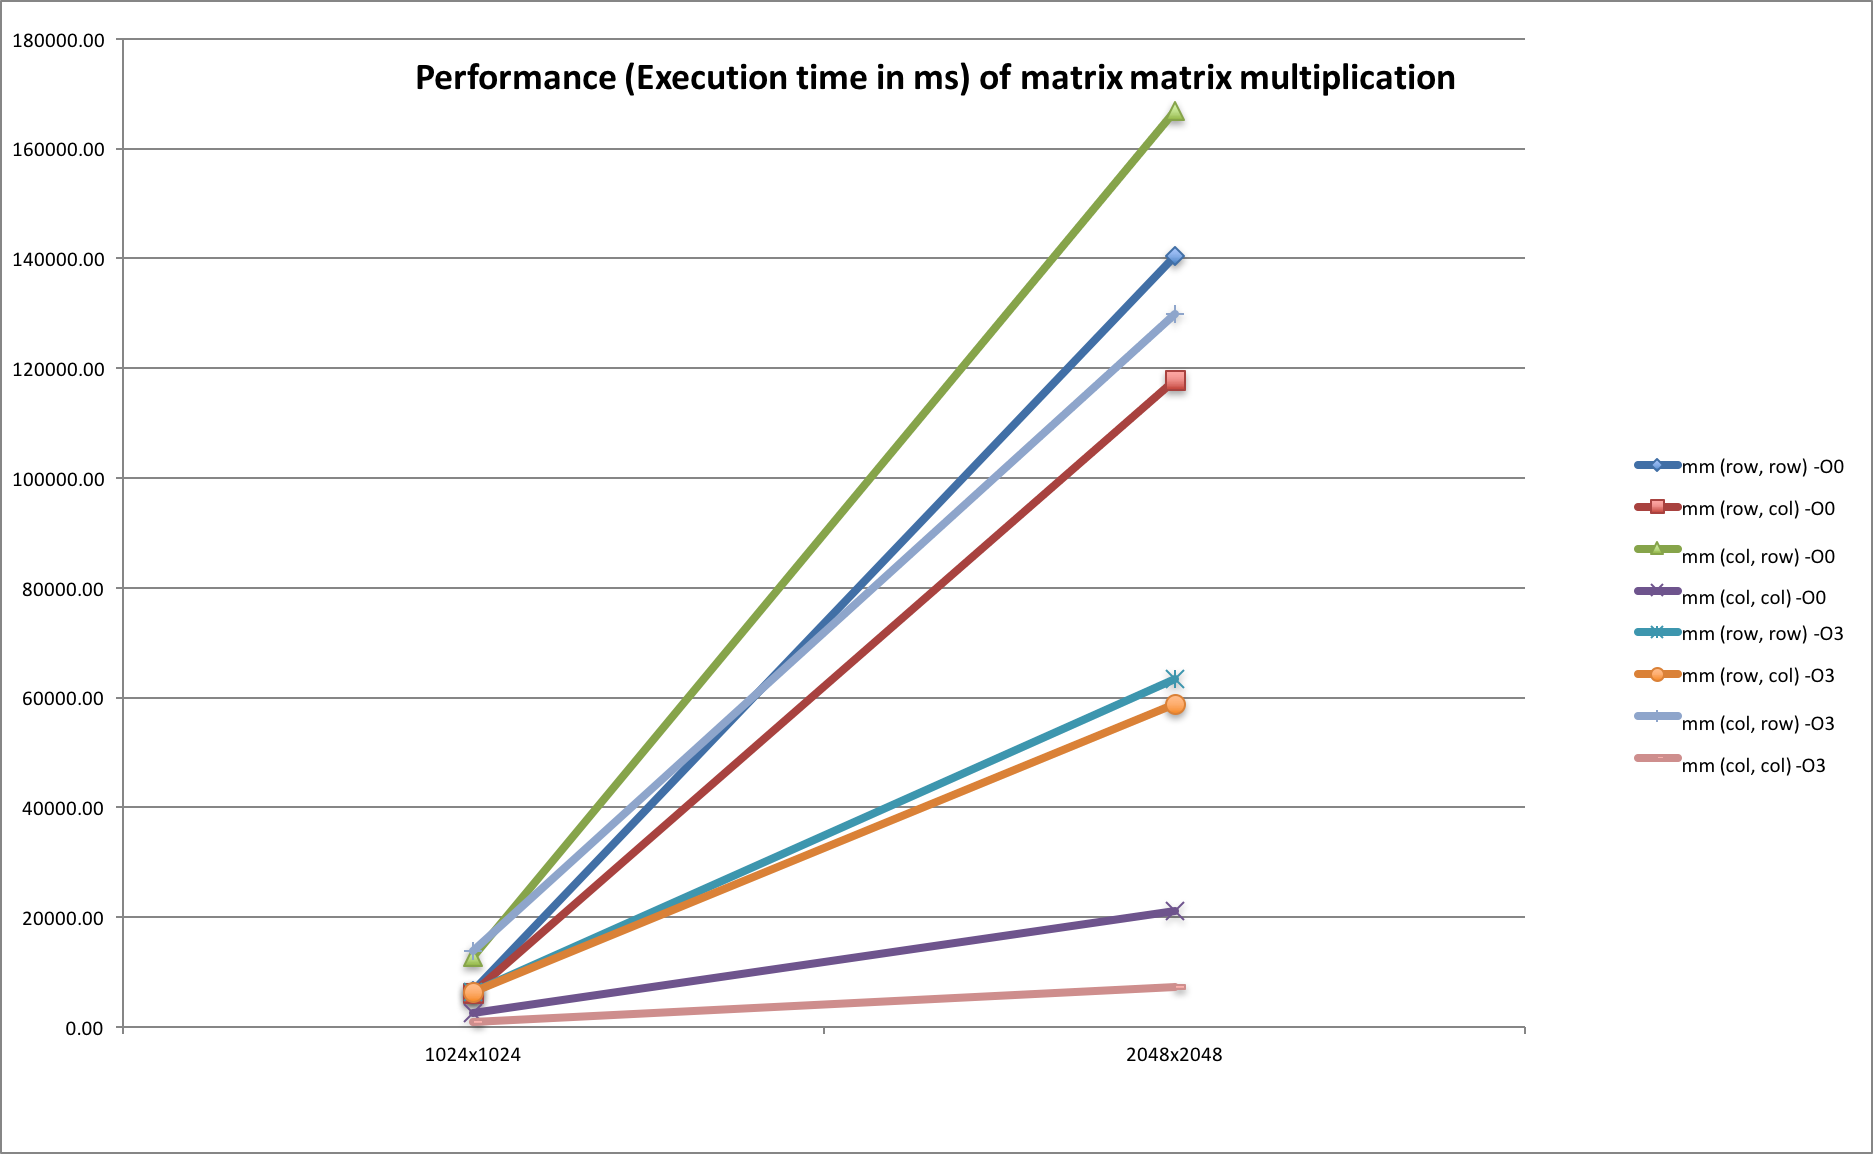
\includegraphics[scale=0.5]{mm.png}}
\vfill
\subfigure[Matrix Vector Performance]{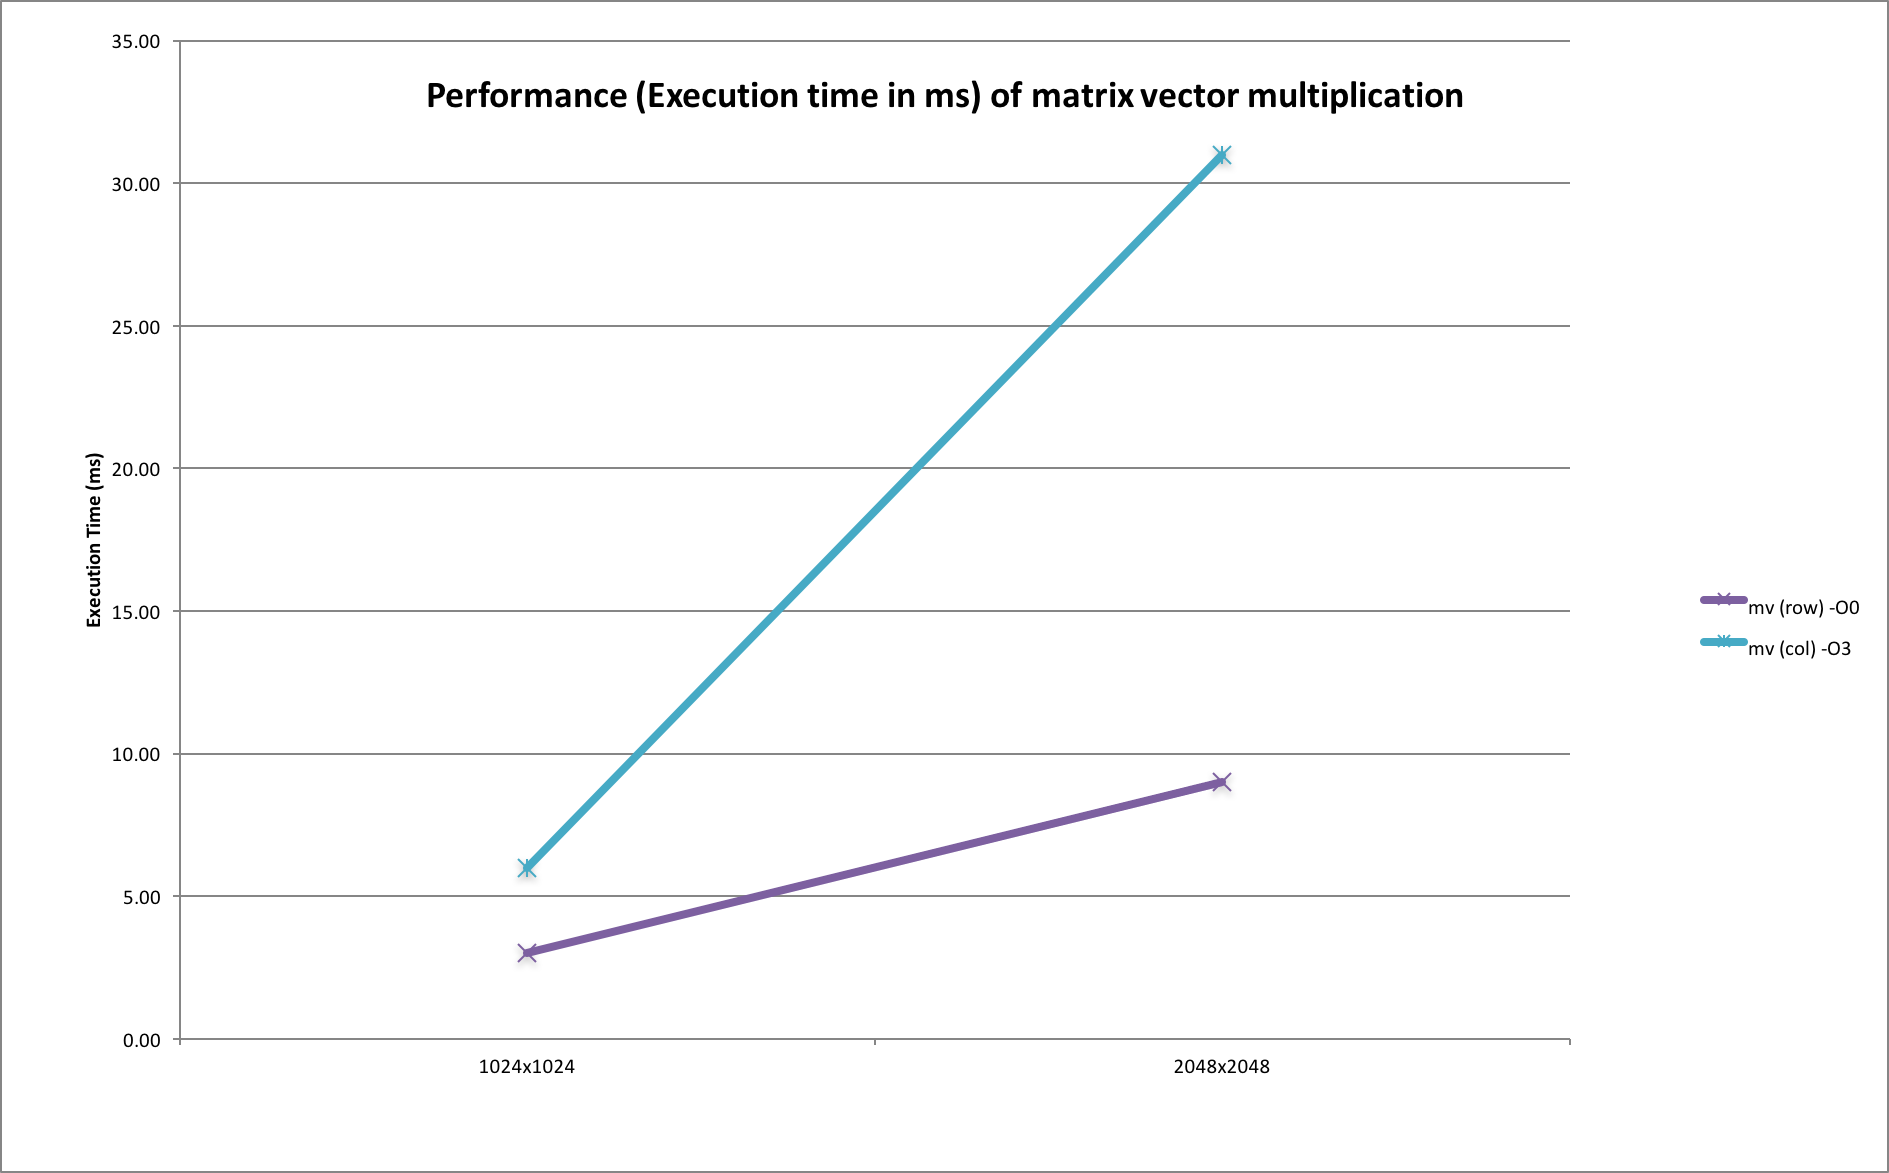
\includegraphics[scale=0.5]{mv.png}}
\vfill
\caption{Performance Graphs}
\end{figure}

\end{document}
              
            
